\subsubsection{Dequantization of mathema\-tics}
\index{Litvinov, Grigory}
\paragraph{Research Team}
Grigory Litvinov (Visiting Professor)

\medskip

%%% give a very short (150 words description of your research area)

  The traditional mathematics over numerical fields can be
dequantized as the Planck constant $\hbar$ tends to zero taking
imaginary values.  This dequantization leads to the so-called
idempotent mathematics based on replacing the usual arithmetic
operations by a new set of basic operations (e.g., such as maximum
or minimum), that is on the concepts of idempotent semifield and
semiring. In the spirit of N. Bohr's correspondence principle in
quantum mechanics there is a correspondence between important,
useful, and interesting constructions and results in the
traditional mathematics and similar results over semifields and
semirings with idempotent addition (the idempotent correspodence
principle). There is an idempotent version
of functional analysis. In particular, a new version of harmonic
analysis and the theory of group representations can be
constructed. For example, the Legendre transform can be treated as
an idempotent version of the Fourier transform.

\paragraph{Highlights}

%%% give a short (500 words)description of the research highlights.
%% 1 figure costs 100 words

My main activity in 2006 was related to a systematic development
of idempotent functional and interval analysis in the framework of
the idempotent correspondence principle. This
principle was formulated by G.L. Litvinov and V.P.
Maslov (Professor Maslov is a founder of idempotent calculus).
A systematic and consistent
application of the correspondence principle leads to a variety of
results, often quite unexpected. A natural passage from the field
of real (or complex) numbers to the so-called max-plus algebra in
mathematical constructions is called a Maslov dequantization. It
corresponds to the well-known Schr\"odinger dequantization for
imaginary values of the Planck constant. There are many
applications of idempotent mathematics, e.g., in mathematical
physics, optimization, geometry, computer science and numerical
methods.

% to include a figure, generate a file xxx.pdf and integrate the
%% following lines
\begin{figure}[ht]
  \begin{center}
    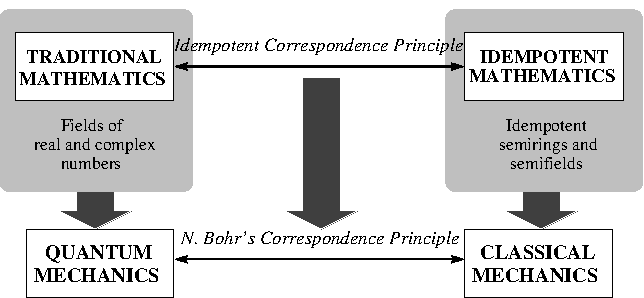
\includegraphics[width=8cm]{Litvinov/Litvinov.pdf}
    \caption{Relations between idempotent and traditional mathematics}
    \label{q:xxx}
  \end{center}
\end{figure}
% to reference it use ``Figure.~\ref{fig:xxx}'';
%% the numbers will be computed automatically.

%In 2006 five of my papers have been published and one paper was
%accepted for publication.

Some investigations were performed with G. B. Shpiz and
A. N. Sbolevski\v i. In particular, we developed and examined
an idempotent version of interval analysis; some new
applications are indicated. An idempotent version
of A. Grothendieck's theory is constructed (nuclear
operators and spaces, kernel theorems etc.).
A new version of the theory of Lipschitz spaces is
developed and relations to idempotent nuclear spaces are
examined. Two survey papers on the subject are
presented.

%Several lectures and conference talks were presented
%(All-Russia Conference ``Interval-06,
%July 1-4, Peterhof, Russia''; Independent University
%of Moscow, Fall 2006).


\paragraph{Organization}
% list the (research) events you have organized, if any,

\begin{enumerate}
%\item  Co-founded the international "Interest group on idempotent
%and tropical mathematics".
\item   An application for scientific cooperation on
idempotent and tropical mathematics between French
and Russian groups in the period 2006--2008.
\end{enumerate}

\paragraph{Collaborations}
\begin{enumerate}
\item {\sl Moscow State University, Russia} \\
  Prof.~V.~Maslov, Prof.~A.~Chebotarev, Dr.~G.~Shpiz, Dr.~A.~Sobolevski\v\i,
  Dr.~S.~Sergeev
\item {\sl Steklov Mathematical Institute, St.~Petersburg, Russia} \\
  Prof.~A.~Vershik
\item {\sl Nottingham Trent University, UK} \\
  Prof.~V.~Kolokoltsov
\item {\sl INRIA, Le Chesnay, France} \\
  Dr.~S.~Gaubert, Dr.~M.~Akian, Prof.~J.-P.~Quadrat
\item {\sl University of Rome-1, Italy} \\
  Dr.~P.~Loreti
\item {\sl Bonn University, Germany} \\
  Prof.~S.~Albeverio, Dr.~A.~Hahn, Dr.~H.~Thaler
\item {\sl University of California, San Diego, USA} \\
  Prof.~W.~McEneany
\item {\sl Universit\'e Louis Pasteur, Strasbourg, France} \\
  Prof.~I.~Itenberg, Prof.~V.~Kharlamov
\item {\sl Lund University, Sweden} \\
  Prof.~I.~Kantor
\end{enumerate}

%\paragraph{Grants}
% list the running grants in 2005, if none have been received, please delete this
% subsection.
%\begin{enumerate}
%\item RFBR grant 05--01--00824 (from the Russian Fund for Basic Research).
%\item RFBR grant 05--01--02807--CNRS.
%\end{enumerate}

\nocite{Litvinov1,Litvinov2,Litvinov3,Litvinov4,Litvinov5,Litvinov6}
